\section{Construction \& Destruction}

RVSDG construction and destruction generate an RVSDG from an input program
and reestablish control flow for code generation, respectively. We present both stages with an
\emph{Inter-Procedure Graph} (IPG) and a CFG as input and output. The IPG is an extension of a
call graph and captures all static dependencies between functions and global variables,
incorporating not only those originating from (direct) calls, but also those from other references
within a function. In the IPG, an edge from node $n1$ to node $n2$ exists, if the body of a
function/global variable corresponding to $n1$ references a function/global variable represented
by $n2$. The utilization of an IPG and a CFG permits a language-independent presentation of RVSDG
construction and destruction.

\subsection{Construction}\label{sec:construction}
RVSDG construction maps all constructs, concepts, and abstractions of an
input language to the RVSDG. The mapping is language-specific, and depends on the language's
features. Languages that permit unstructured control flow, such as C
or C++, cannot be mapped directly to the RVSDG and require a CFG as a stepping
stone, while languages such as Haskell permit direct construction~\cite{Reissmann12}.
In this section, we present RVSDG construction for the former case as it
encompasses the latter.
Conceptually, RVSDG construction can be split in two phases:

\begin{enumerate}
	\item \textit{Inter-Procedural Translation} (Inter-PT) translates functions, global variables,
	and inter-procedural dependencies, creating \lambdam, \deltam, and \phinodes.

	\item \textit{Intra-Procedural Translation} (Intra-PT) translates intra-procedural
		control and data flow, creating a \deltam/\lambdaregion from a function's/global variables'
		body.
\end{enumerate}

Inter-PT invokes Intra-PT for each function's or global variables' body, and both
phases interact through a common symbol table. The table maps function and CFG variables to
RVSDG arguments or outputs, and is updated with every creation of a
node or region. We omit the updates from our algorithm descriptions for brevity.

\subsubsection{Inter-Procedural Translation}\label{sec:interproc}

Inter-PT converts all functions and global variables from the \emph{Inter-Procedure Graph} (IPG) of
a translation unit to \lambdanodes and \deltanodes, respectively. Figure~\ref{fig:exp-ipg-ipg}
shows the IPG for the code in Figure~\ref{fig:exp-ipg-code}. The code
consists of four functions, with function \verb;sum; performing two indirect calls. The
corresponding IPG consists of four nodes and three edges. All edges originate from node $tot$, as
it is the only function that explicitly references other functions, \ie \verb;sum; for a direct
call, and \verb;f; and \verb;g; to pass as argument. No edge originates from node \verb;sum;, as
the corresponding function does not explicitly reference any other functions, and the functions for
the indirect calls are provided as arguments.

The RVSDG puts two constraints on the translation from an IPG. Firstly, mutually recursive entities
are required to be created within \phinodes to preserve the RVSDG's acyclicity. Secondly, Inter-PT
must respect the calling dependencies of functions to ensure that \lambdanodes are created before
their \applynodes. In order to embed mutually recursive entities into \phinodes, we need to
identify the strongly connected components (SCCs) in the IPG. We consider an SCC
\emph{trivial}, if it consists only of a single node with no self-referencing edges. Otherwise, it
is \emph{non-trivial}. Moreover, a trivial SCC might not have a CFG associated with it, and is
therefore defined in another translation unit.

\begin{figure*}
	\subfloat[Code\label{fig:exp-ipg-code}] {
		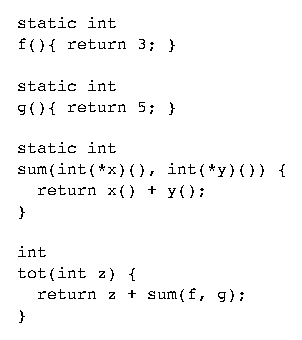
\includegraphics[scale=0.84]{ipg-code}
	}
	\hfill
	\subfloat[IPG\label{fig:exp-ipg-ipg}] {
		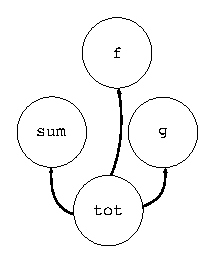
\includegraphics[scale=0.84]{ipg}
	}
	\hfill
	\subfloat[RVSDG\label{fig:exp-ipg-rvsdg}] {
		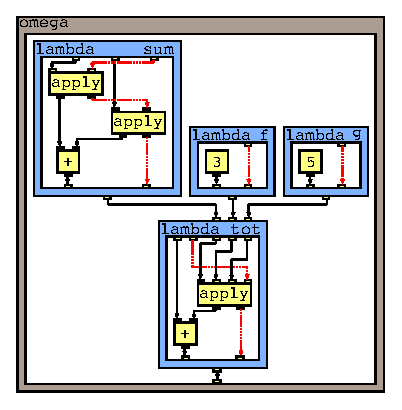
\includegraphics[scale=0.84]{ipg-rvsdg}
	}
	\caption{Inter-Procedural Translation}
	\label{fig:exp-ipg}
\end{figure*}

\begin{informalg}{Inter-Procedural Translation}{alg:interpt}
Compute all SCCs in an IPG and process them in topological order of the directed acyclic
graph formed by the SCCs as follows:
	\begin{enumerate}
		\item \label{item:trivial} \bpoint{Trivial SCC}:
			\begin{enumerate}
				\item \bpoint{Function with CFG}: Begin a \lambdanode by adding all context variables,
					function arguments, and an additional state argument to the \lambdaregion. Translate the
					CFG with Intra-PT as explained in Section~\ref{sec:intraproc}, and finish the
					\lambdanode by adding the function results and the state result to the
					\lambdaregion. If a function is exported, add a result to the \omegaregion and connect
					the \lambdanode's output to it.

				\item \bpoint{Global variable with CFG}: Begin a \deltanode by adding all context variables
					to the \deltaregion. Translate the CFG with Intra-PT as eplained in
					Section~\ref{sec:intraproc}, and finish the \deltanode by adding the result to the
					\deltaregion. If a global variable is exported, add a result to the \omegaregion and
					connect the \deltanode's output to it.

				\item \bpoint{Without CFG}: Add a \omegaregion argument for the external entity.
			\end{enumerate}

		\item \label{item:non-trivial} \bpoint{Non-trivial SCC}: Begin a \phinode by adding all
			functions/global variables as well as context variables to the \phiregion. Translate each
			entity in the SCC according to \textsc{Trivial SCC} without exporting them. Finish the
			\phinode by adding all outputs as results to the \phiregion. If an entity is exported, add a
			result to the \omegaregion and connect the \phinode's output to it.
		\vspace*{-\baselineskip}
	\end{enumerate}
\end{informalg}

Algorithm~\ref{alg:interpt} outlines the RVSDG construction from an IPG. It finds all SCCs
and converts trivial SCCs to individual \deltam/\lambdanodes, while the \deltam/\lambdanodes
created from non-trivial SCCs are embedded in \phinodes. This satisfies the first constraint. The
second
constraint is satisfied by processing SCCs in topological order, creating \lambdanodes before their
\applynodes. Identification and ordering of SCCs can be done in a single step with
Tarjan's algorithm~\cite{Tarjan72}, which returns identified SCCs in reverse topological order.
Figure~\ref{fig:exp-ipg-rvsdg} shows the RVSDG after application of Algorithm~\ref{alg:interpt}
to the IPG in Figure~\ref{fig:exp-ipg-ipg}. In addition to a function's arguments,
Algorithm~\ref{alg:interpt} adds a state argument and result to \lambdaregions (the
red dashed line in Figure~\ref{fig:exp-ipg-rvsdg}), to sequence stateful computations.
Nodes representing operations with
side-effects consume this state and produce a new state for the next node.

\subsubsection{Intra-Procedural Translation}\label{sec:intraproc}
The RVSDG puts several constraints on the translation of intra-procedural control and data flow.
Firstly, it requires that the control flow only consists of constructs that can be translated to
\gammam and \thetanodes, \ie it can only consist of tail-controlled loops and conditionals with
symmetric control flow splits and joins. Secondly, the nesting and relation of these
constructs to each other is required as the RVSDG is a hierarchical representation. Thirdly, it is
necessary to know the data dependencies of these structures in order to construct \gammam and
\thetanodes. While these constraints are beneficial for optimizations by substantially simplifying
their implementation%
, they render RVSDG construction non-trivial.

This section's construction algorithm enables the translation of any data and control flow,
irregardless of its complexity, to the RVSDG. It creates a \deltam/\lambdaregion from a global
variables' or function's body in four stages:

\begin{enumerate}
	\item \textit{Control Flow Restructuring} (CFR) restructures a CFG to make
		it amenable to RVSDG construction.

	\item \textit{Structural Analysis} constructs a control tree~\cite{Muchnick97} from the
		restructured CFG, discovering the CFG's individual control flow regions.

	\item \textit{Demand Annotation} annotates the discovered control flow regions with the
		variables that are demanded by the instructions within these regions.

	\item \textit{Control Tree Translation} converts the annotated control tree into a
		\deltam/\lambdaregion.
\end{enumerate}

CFR ensures the first requirement by translating a function's control flow to a form that is
amenable to RVSDG construction. It restructures control flow to a form that enables the direct
mapping of a CFG's control flow regions to the RVSDG's \gammam and \thetanodes. CFR can be omitted
for languages with limited control flow structures, such as Haskell or Scheme. Structural analysis
ensures the second requirement by constructing a control tree from the CFG, exposing the control
regions nesting and the relation to each other. Demand annotation fulfills the third requirement
by annotating the control tree's nodes with their data dependencies. Finally, the annotated control
tree can be translated to a \deltam/\lambdaregion. The rest of this section covers the four stages
in detail.

\paragraph{Control Flow Restructuring:}
CFR converts a CFG to a form that only contains tail-controlled loops and conditionals with
properly nested splits and joins. This stage is only necessary for languages that support more
complex control flow constructs, such as \verb;goto; statements or short-circuit operators, but
can be omitted for languages with more limited control flow. CFR consists of two interlocked
phases: loop restructuring and branch restructuring. Loop restructuring transforms all loops to
tail-controlled loops, while branch restructuring ensures conditionals with symmetric control flow
splits and joins.

We omit an extensive discussion of CFR as it is detailed in Bahmann~\etal~\cite{Bahmann15}.
In contrast to node splitting approaches~\cite{Zhang04}, CFR avoids the possibility of exponential
code blowup~\cite{Carter03} by inserting additional predicates and branches instead of cloning
nodes. Moreover, it does not require a CFG in SSA form as this form is automatically established
throughout construction.


\paragraph{Structural Analysis:}
After CFR, a restructured CFG consists of 3 single-entry/single-exit control flow regions:

\begin{itemize}
	\item \textit{Linear Region}: A linear subgraph where the entry node and all intermediate nodes
		have only one outgoing edge, and the exit node as well as all intermediate nodes have only one
		incoming edge.

	\item \textit{Branch Region}: An subgraph with the entry and exit node representing the
		control flow split and join, respectively, and each branch alternative consisting of a single
		node.

	\item \textit{Loop Region}: A single node where an edge originates and targets this node.
\end{itemize}

These control flow regions and their corresponding nesting structure can be exposed by performing
an interval~\cite{Muchnick97} or structural~\cite{Sharir80} analysis. The analysis result is a
control tree~\cite{Muchnick97} with basic blocks as leaves and abstract nodes representing the
control flow regions as branches.

A linear region maps to a \emph{linear node} in the control tree with the
linear subgraph's entry and exit node as the node's left and right most child, respectively.
A branch region maps to two control tree nodes: a \emph{branch node} and a linear node. The branch
node represents the region's alternatives with the corresponding nodes as its children.
A linear node with three children can then be used to capture the rest of the branch region. Its
first child is the region's entry node, the second child the branch node representing the
alternatives, and the third child the region's exit node. Finally, a loop region maps to a
\emph{loop node} with the region's single node as its child.

Figure~\ref{fig:euclid_cfg} shows Euclid's algorithm as a CFG, and
Figure~\ref{fig:euclid_restructured} shows the same CFG after CFR, which restructured the
head-controlled loop to a tail-controlled loop. The left of Figure~\ref{fig:euclid_pst} shows
the corresponding control tree. %

\begin{figure*}
	\subfloat[CFG\label{fig:euclid_cfg}]{
		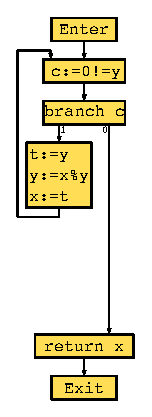
\includegraphics[scale=0.84]{euclid_cfg}
	}
	\hfill
	\subfloat[Restructured CFG\label{fig:euclid_restructured}]{
		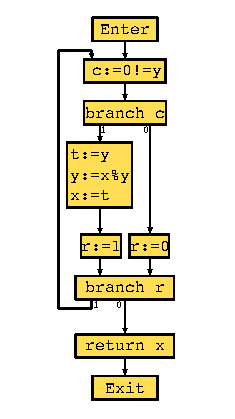
\includegraphics[scale=0.84]{euclid_restructured}
	}
	\hfill
	\subfloat[Annotated control tree\label{fig:euclid_pst}]{
		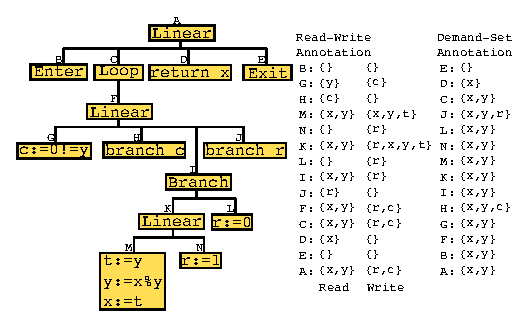
\includegraphics[scale=0.84]{euclid_pst}
	}
	\hfill
	\subfloat[RVSDG\label{fig:euclid_rvsdg}]{
		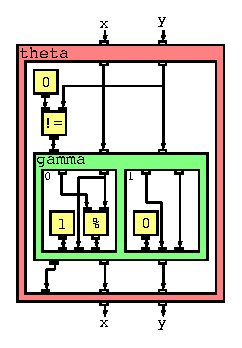
\includegraphics[scale=0.84]{euclid_rvsdg}
	}
	\caption{Intra-Procedural Translation}
	\label{fig:euclid}
\end{figure*}

\paragraph{Demand Annotation:}
Structural analysis exposes necessary control flow regions for a direct translation to
RVSDG. A control flow tree's branch and loop nodes map directly to \gammam and
\thetanodes, and individual instructions to simple nodes, but it is further
necessary to expose the data dependencies of these nodes for efficient generation.

This is the task of demand annotation. It exposes these data dependencies by annotating control
tree nodes with the variables that are demanded by the instructions within control flow regions.
It accomplishes this using a \emph{read-write} and \emph{demand-set} annotation pass.
The read-write pass annotates each control tree node with the set of read and written variables of
the corresponding control flow region, while the demand-set pass uses these variables
to annotate each control tree node with the set of demanded variables, \ie variables that are
necessary to fulfill the dependencies of the instructions within a control flow region.

\begin{informalg}{Demand Annotation}{alg:da}
\begin{enumerate}
	\vspace*{-0.7\baselineskip}

	\item \bpoint{Read-Write Annotation}: Process the control tree nodes in post-order as follows:
		\begin{itemize}
			\item \bpoint{Basic Block}: For each instruction $i$ processed bottom-up, the read set is
				$R = (R \setminus W_i) \cup R_i$. The write set is $W = \bigcup W_i$.

			\item \bpoint{Linear Node}: For each child $c$ processed right to left, the read set is
				$R = (R \setminus W_c) \cup R_c$. The write set is $W = \bigcup W_c$.

			\item \bpoint{Branch Node}: For each child $c$, the read set and write set is
				$R = \bigcup R_c$ and $W = \bigcap W_c$, respectively.

			\item \bpoint{Loop Node}: For the child $c$, the read set and write set is $R = R_c$ and
				$W = W_c$, respectively.
		\end{itemize}

	\item \bpoint{Demand-Set Annotation}: Process the control tree nodes with an empty demand set
		$D_t$ as follows:
		\begin{itemize}
			\item \bpoint{Basic Block}: Set $D = D_t = (D_t \setminus W) \cup R$ and continue processing.

			\item \bpoint{Linear Node}: Recursively process the children right to left.
				Set $D = D_t = (D_t \setminus W) \cup R$. and continue processing.

			\item \bpoint{Branch Node}: Set $D_{tmp} = D_t$. Recursively process each child with a copy
				of $D_t$. Set $D = D_t = (D_{tmp} \setminus W) \cup R$ and continue processing.

			\item \bpoint{Loop Node}: Set $D = D_t \cup R$. Recursively process the child with
				$D_t = D$ and continue processing.
		\end{itemize}

	\vspace*{-\baselineskip}
\end{enumerate}
\end{informalg}

Algorithm~\ref{alg:da} shows the details of the two passes. The read-write pass annotates each node
with the read set $R$ and write set $W$. It processes the tree in post-order, building up
the two sets from the innermost to the outermost nested control flow region. For linear nodes, the
children are processed from right to left, \ie bottom-up in the restructured CFG, to create the
two sets. For branch nodes, a variable is only considered to be written, if it is in the write
set of \emph{all} the node's children, \ie it was written in all alternatives of a conditional.

The demand-set pass uses the read set $R$ and write set $W$ to construct a demand set $D$ for each
node. The algorithm is initialized with an empty set $D_t$, which is used to keep track of
demanded variables during traversal. The demand-set pass traverses the tree such that it follows
a bottom-up traversal of the restructured CFG, adding and removing variables from $D_t$ during
this traversal according to each node's rules. For branch nodes, each child is processed with a copy of
$D_t$, as the corresponding alternatives of the conditional are independent from another. For loop
nodes, the \thetanode's requirement that inputs and outputs must have the same signature
necessitates that $R$ is added to $D_t$ \emph{before} the loop's body is processed.
The right of Figure~\ref{fig:euclid_pst} shows the traversal order for the two passes along with
the read, write, and demand set for each node of the control tree on the left.

\paragraph{Control Tree Translation:}
After demand annotation, each node of the control tree is annotated with the set of variables that
its instructions require, \ie their data dependencies. Finally, the control tree translation
constructs a \deltam/\lambdaregion from the control tree along with its annotated demand sets.
Algorithm~\ref{alg:st} shows the details. The algorithm processes each node in the control tree
creating \gammam and \thetanodes for all branch and loop nodes, respectively.
It uses the demand set of the right sibling for the outputs of gamma nodes,
corresponding to the branch region's join node in the CFG.
Figure~\ref{fig:euclid_rvsdg} shows the resulting RVSDG nodes for the example.

\begin{informalg}{Control Tree Translation}{alg:st}
Process the control tree nodes as follows:
\begin{itemize}
	\item \bpoint{Basic Block}: Process the node's operations top-down creating simple nodes in the
		RVSDG.

	\item \bpoint{Linear Node}: Recursively process the node's children top-down.

	\item \bpoint{Branch Node}:Begin a \gammanode with inputs according to the node's demand set.
		Create subregions by recursively processing the node's children. Finish the \gammanode with
		outputs according to its right sibling node's demand set.

	\item \bpoint{Loop Node}: Begin a \thetanode with inputs according to the node's demand set.
		Create its region by recursively processing its child. Finish the \thetanode with outputs
		according to its demand set.

	\vspace*{-\baselineskip}
\end{itemize}
\end{informalg}

\subsubsection{Modeling Stateful Computations}\label{sec:modeling-state}
Algorithm~\ref{alg:interpt} adds an additional state argument and result to every \lambdanode. This
state is used to sequentialize all stateful computations within a function. Nodes
with side-effects consume this state and produce a new state for consumption by the next node. This
single state ensures that the order of operations with side-effects in the RVSDG is according to
the total order specified in the original program, ensuring correct observable behavior.
Specifically, the use of a single state for sequentializing stateful operations ensures that the
order of these operations in the RVSDG is equivalent to the order in the restructured CFG.

The utilization of a single state is, however, overly
conservative, as different computations can have mutually exclusive side-effects. For example, the
side-effect of a non-terminating loop is unrelated to a non-dereferencable load. These stateful
computations can be modeled independently with the help of distinct states, as depicted in
Figure~\ref{fig:exp2-rvsdg}. This results in the explicit exposure of more concurrent computations,
as loops with no memory operations would become independent from other loops with memory
operations. Moreover, the possibility of encoding independent states can also be leveraged by
analyses and optimizations. For example, alias analysis can directly encode independent memory
operations into the RVSDG by introducing additional memory states. Pure functions could
be easily recognized and optimized, as they would contain no operations that use the added states
and therefore would only pass it through, \ie, the origin of the state result would be the
\lambdaregion's argument.


